\lstset{style=mystyle}

\section{Implementation}
\label{sec:implementation}

\subsection{Introduction}
\label{subsec:introduction}

This chapter provides a detailed walkthrough of the implementation process for the Student Portal project. The platform is structured into four major components: the backend server, web application, mobile application, and AI/ML services. Each component is managed collaboratively via our GitHub organization using issue tracking, pull requests, and continuous integration.

\subsubsection{System Architecture Highlights}

\begin{itemize}
    \item \textbf{Backend:} Node.js with TypeScript, following a repository-service-controller pattern. Mongoose handles the database layer, and the codebase is organized into modular folders.
    
    \item \textbf{Web Application:} Built with Next.js and styled with Tailwind CSS. Uses TanStack Query for state management and React Hook Form for form handling.
    
    \item \textbf{Mobile Application:} Built in Flutter with a clean architecture using the BLoC pattern. Each feature has its own folder containing BLoC, use cases, UI, and data layer.
    
    \item \textbf{AI/ML Services:} Python-based services using PyTorch, FAISS, and Flask. Modular design separates chatbot, recommendation, and inference code.
\end{itemize}

\subsection{GitHub Organization and Workflow}
\label{subsec:github_workflow}

Our project is managed through a dedicated GitHub organization that serves as the central hub for collaboration, code management, and project tracking. The organization structure and workflow are designed to facilitate efficient team collaboration and maintain high code quality standards.

\subsubsection{Organization Structure}
\label{subsubsec:org_structure}

The GitHub organization is organized into several key repositories:

\begin{itemize}
    \item \textbf{student-portal-server}: Backend server implementation
    \item \textbf{student-portal-web}: Next.js web application
    \item \textbf{student-portal-app}: Flutter mobile application
    \item \textbf{student-portal-ai}: AI/ML models and services
    \item \textbf{student-portal-docs}: Project documentation and guides
\end{itemize}

\begin{figure}[h]
    \centering
    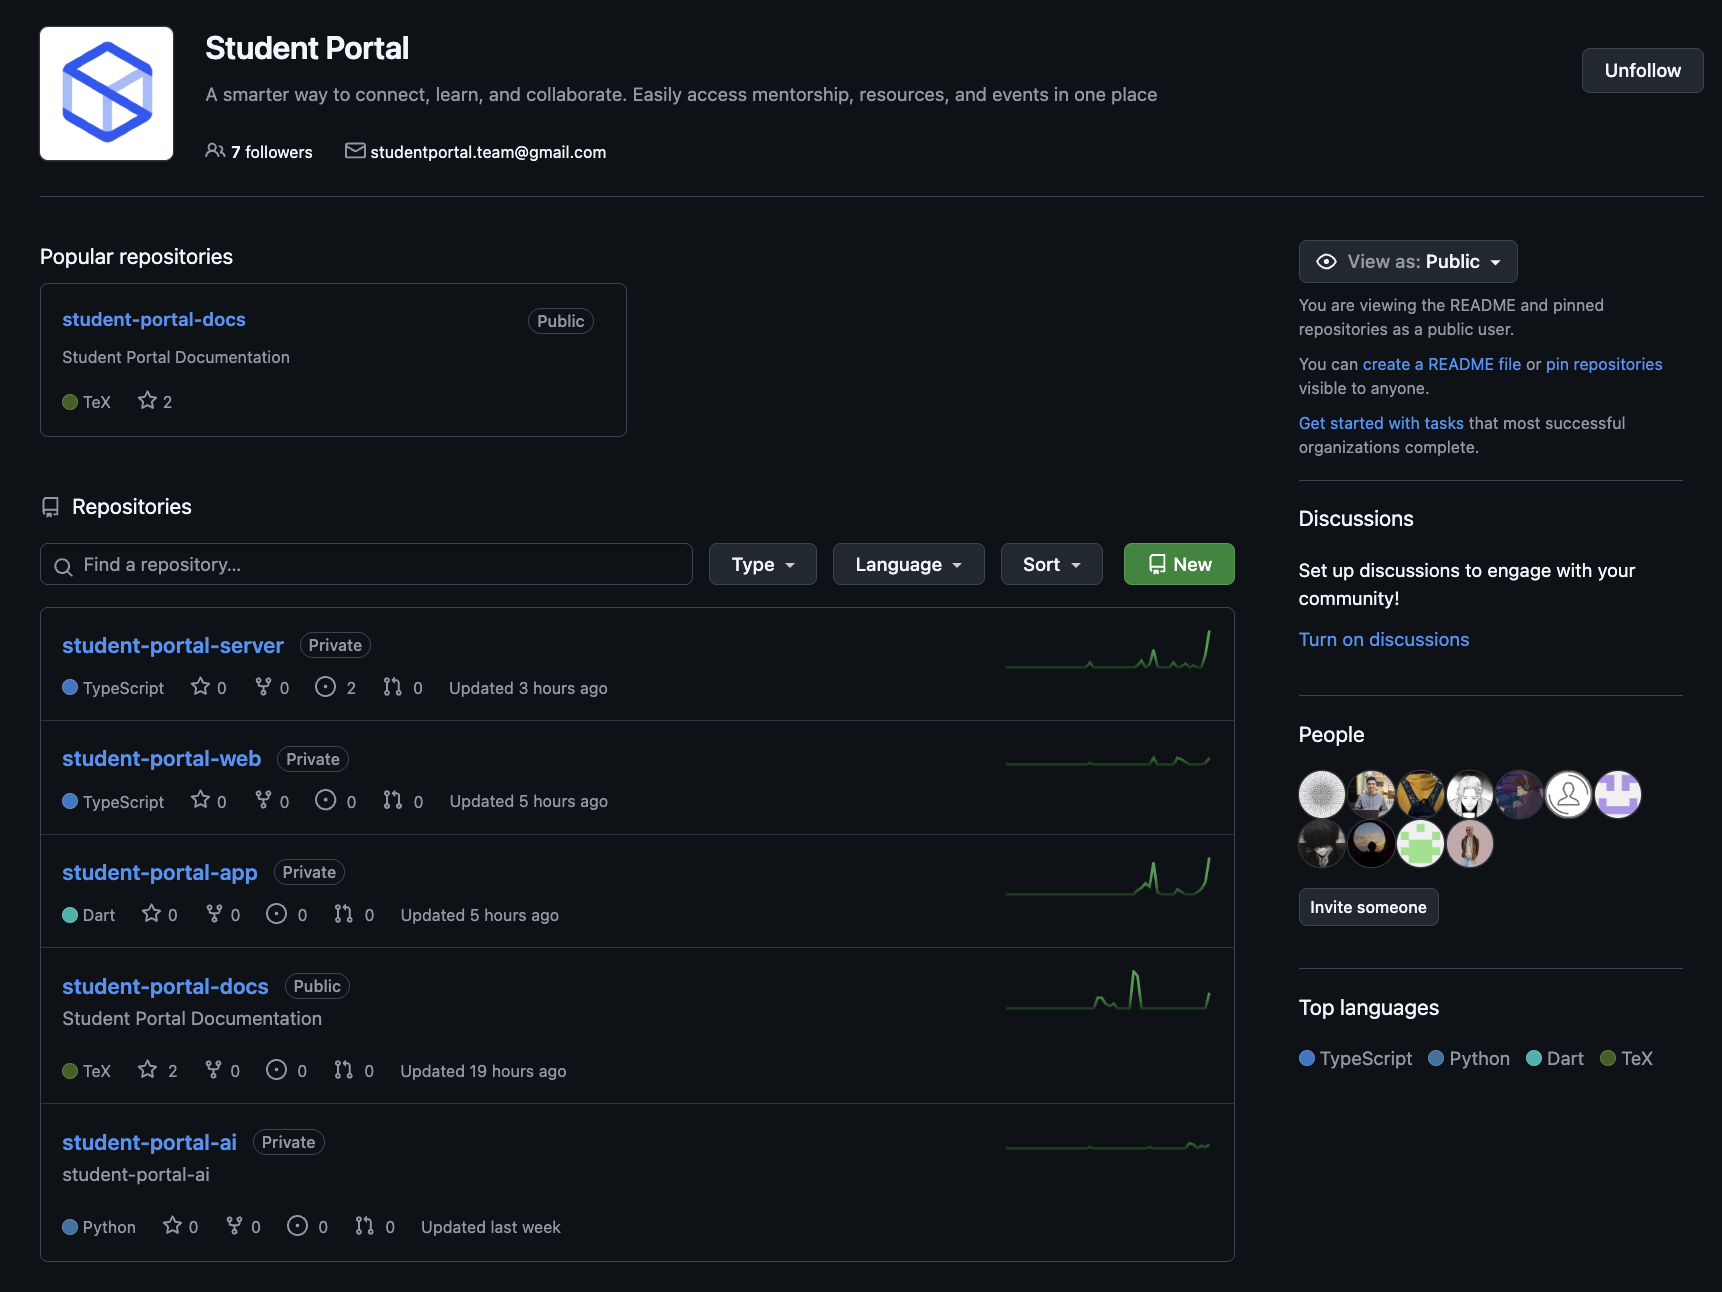
\includegraphics[width=0.8\textwidth]{images/github-org-overview}
    \caption{GitHub Organization Overview}
    \label{fig:github_org}
\end{figure}

\subsubsection{Development Workflow}
\label{subsubsec:dev_workflow}

Our development process is built on efficient collaboration and high-quality standards. We maintain a structured Git workflow with clear branching strategies and automated pipelines. Discord meetings keep the team aligned, while our comprehensive documentation ensures smooth knowledge sharing. The combination of agile practices and automated testing allows us to deliver features while maintaining code quality.

\subsection{Frontend Screens}
\label{subsec:frontend_screens}

\subsubsection{Web Application Screens}
\label{subsubsec:web_screens}

\begin{itemize}
    \item \textbf{Student Dashboard:} A modern, responsive dashboard with activity feed, quick access to events, performance metrics, and personalized recommendations.
    
    \item \textbf{Event Management Portal:} Interactive calendar interface with event creation wizard, attendee management, and automated notifications.
    
    \item \textbf{Community Hub:} Member directory with role management, discussion forums, and resource sharing capabilities.
    
    \item \textbf{AI Learning Assistant:} Real-time chat interface with progress tracking and personalized study recommendations.
\end{itemize}

% Web Application Screenshots
\begin{figure}[h]
    \centering
    \begin{subfigure}[b]{0.45\textwidth}
        \centering
        % \includegraphics[width=\textwidth]{images/web-dashboard.png}
        \caption{Student Dashboard}
        \label{fig:web-dashboard}
    \end{subfigure}
    \hfill
    \begin{subfigure}[b]{0.45\textwidth}
        \centering
        % \includegraphics[width=\textwidth]{images/web-events.png}
        \caption{Event Management}
        \label{fig:web-events}
    \end{subfigure}
    \vskip\baselineskip
    \begin{subfigure}[b]{0.45\textwidth}
        \centering
        % \includegraphics[width=\textwidth]{images/web-community.png}
        \caption{Community Hub}
        \label{fig:web-community}
    \end{subfigure}
    \hfill
    \begin{subfigure}[b]{0.45\textwidth}
        \centering
        % \includegraphics[width=\textwidth]{images/web-ai-assistant.png}
        \caption{AI Learning Assistant}
        \label{fig:web-ai}
    \end{subfigure}
    \caption{Web Application Screens}
    \label{fig:web_screens}
\end{figure}

\subsubsection{Mobile Application Screens}
\label{subsubsec:mobile_screens}

\begin{itemize}
    \item \textbf{Home Feed:} Personalized mobile dashboard with swipeable activity cards and quick actions.
    
    \item \textbf{Event Explorer:} Location-aware event discovery with one-tap registration and offline support.
    
    \item \textbf{Smart Search:} Voice-enabled search with real-time suggestions and category filtering.
    
    \item \textbf{Messaging Center:} Real-time messaging with file sharing and media preview capabilities.
\end{itemize}

% Mobile Application Screenshots
\begin{figure}[H]
    \centering
    \begin{subfigure}[b]{0.22\textwidth}
        \centering
        % 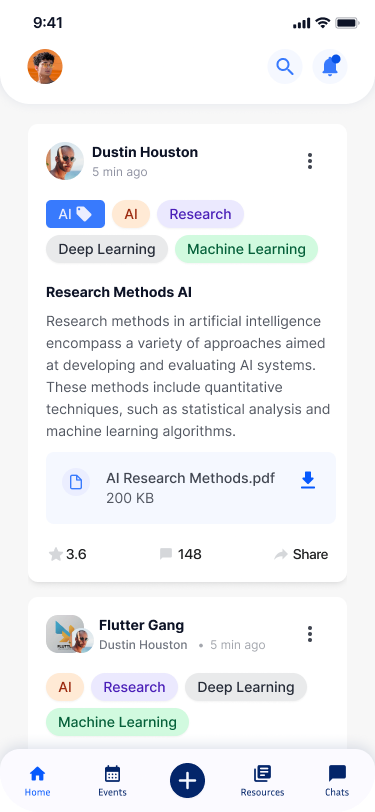
\includegraphics[width=\textwidth,height=0.3\textheight,keepaspectratio]{images/mobile-home.png}
        \caption{Home Feed}
        \label{fig:mobile-home}
    \end{subfigure}
    \hfill
    \begin{subfigure}[b]{0.22\textwidth}
        \centering
        % 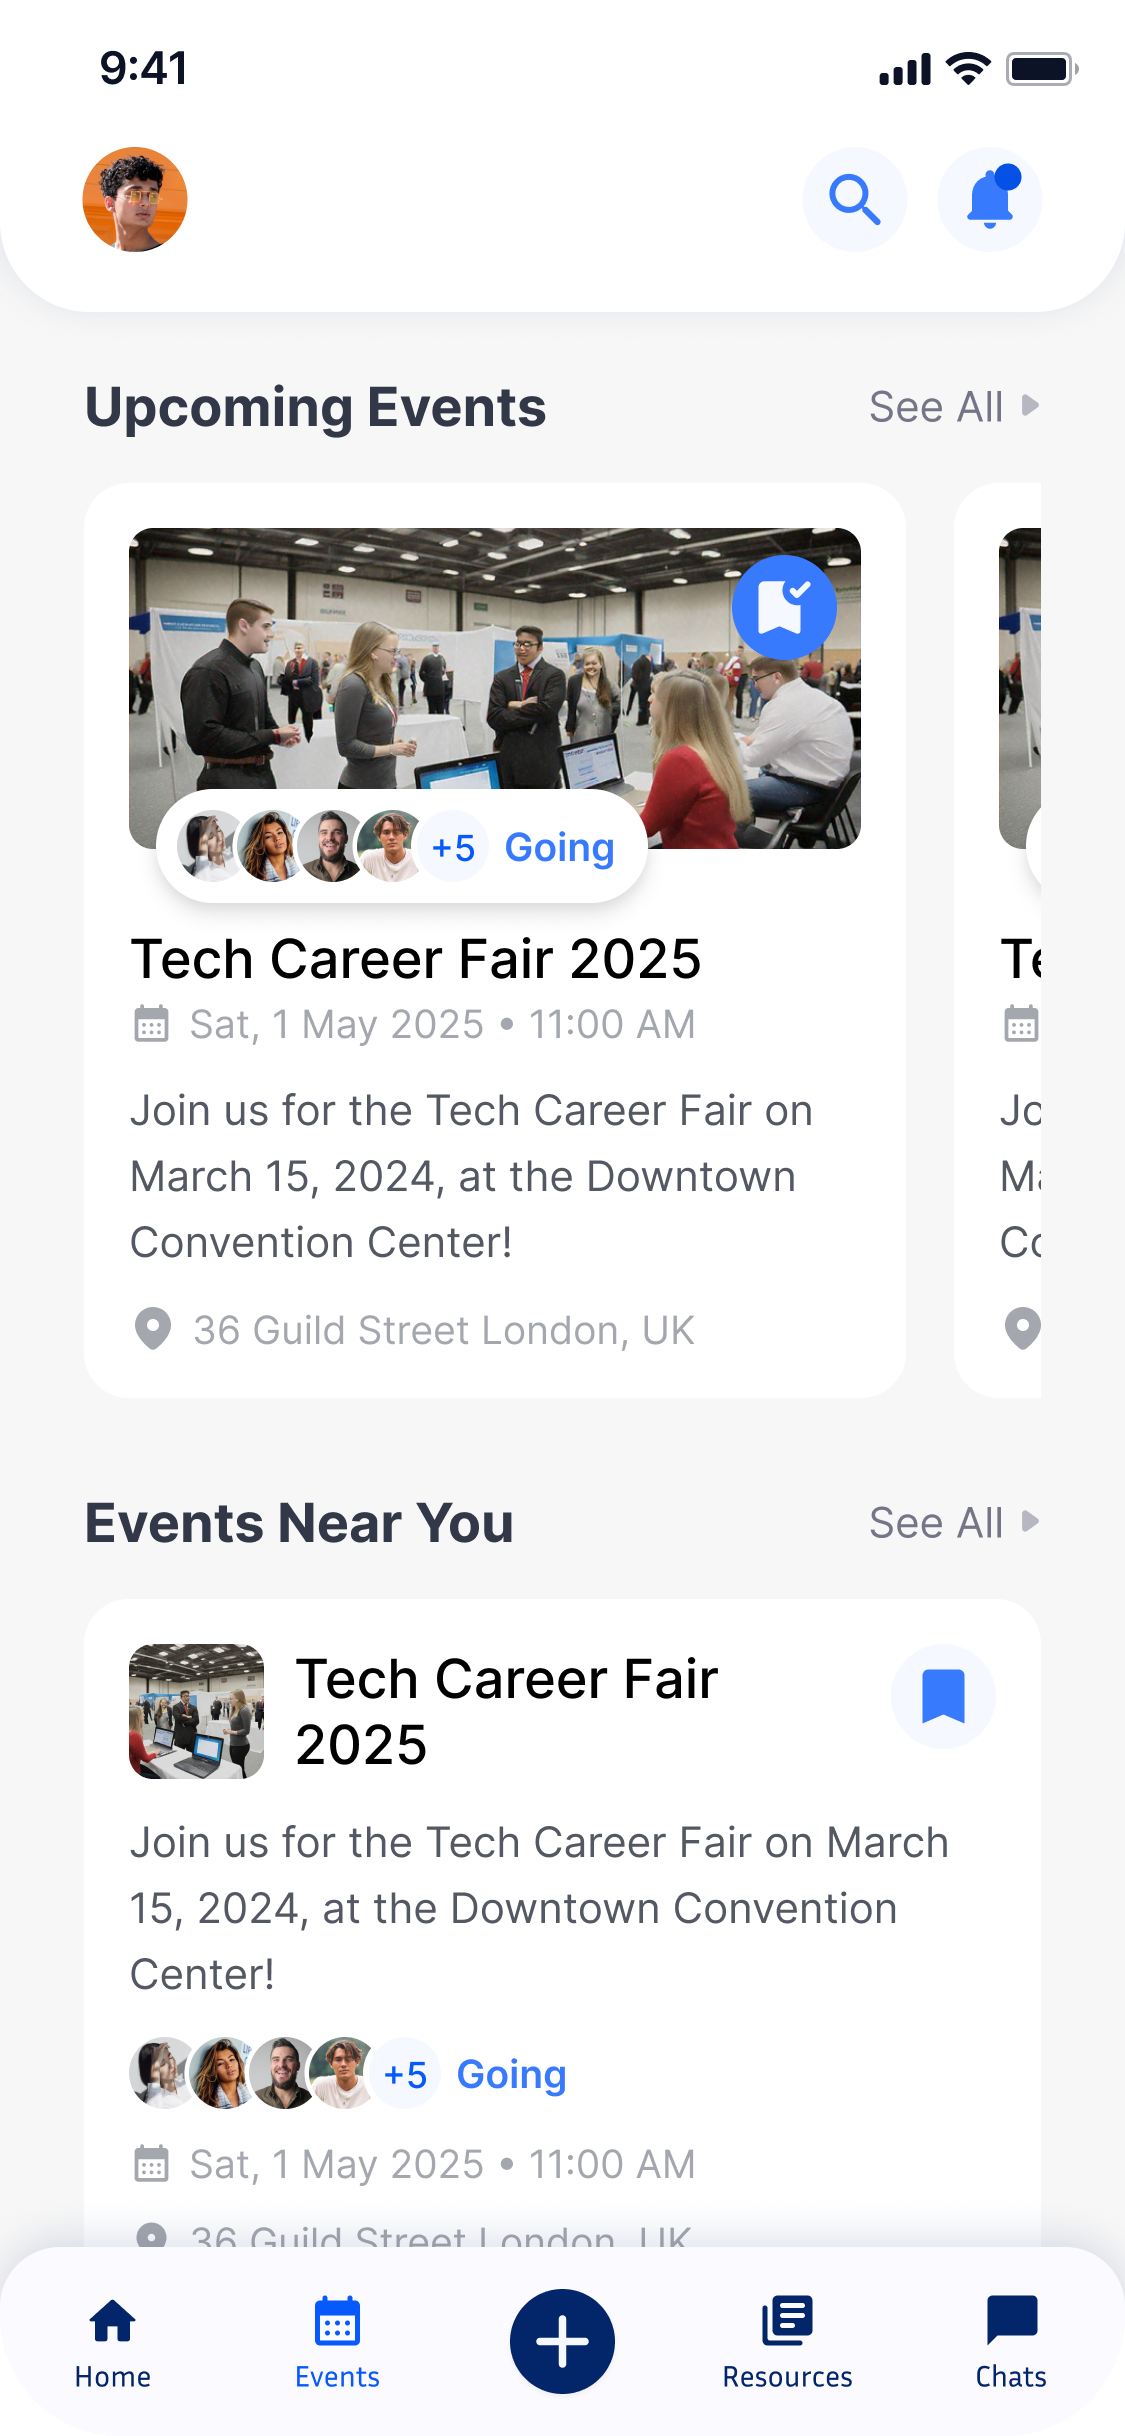
\includegraphics[width=\textwidth,height=0.3\textheight,keepaspectratio]{images/mobile-events.png}
        \caption{Event Explorer}
        \label{fig:mobile-events}
    \end{subfigure}
    \hfill
    \begin{subfigure}[b]{0.22\textwidth}
        \centering
        % \includegraphics[width=\textwidth,height=0.3\textheight,keepaspectratio]{images/mobile-search.png}
        \caption{Smart Search}
        \label{fig:mobile-search}
    \end{subfigure}
    \hfill
    \begin{subfigure}[b]{0.22\textwidth}
        \centering
        % \includegraphics[width=\textwidth,height=0.3\textheight,keepaspectratio]{images/mobile-messaging.png}
        \caption{Messaging Center}
        \label{fig:mobile-messaging}
    \end{subfigure}
    \caption{Mobile Application Screens}
    \label{fig:mobile_screens}
\end{figure}

Each screen is designed with a focus on user experience, accessibility, and performance. The interfaces follow material design principles and maintain consistency across platforms while adapting to the unique capabilities of each device type.

\subsection{Project File Structure Overview}
\label{subsec:file_structure}

Below is the structured layout of each major component of the Student Portal project, showing the first two levels of the directory structure:

\subsubsection{Backend (Node.js + TypeScript)}

\begin{lstlisting}[language=bash, caption={Backend Directory Structure (tree -L 2)}]
backend/
├── __tests__/
├── docs/
├── src/
│   ├── config/          # Environment and app configuration
│   ├── controllers/     # Request handlers and route logic
│   ├── interfaces/      # TypeScript type definitions
│   ├── libs/           # Third-party library integrations
│   ├── middleware/     # Express middleware functions
│   ├── models/         # Mongoose schema definitions
│   ├── repositories/   # Data access layer
│   ├── routes/         # API route definitions
│   ├── services/       # Business logic layer
│   ├── types/          # Custom type definitions
│   ├── utils/          # Helper functions
│   └── validators/     # Input validation schemas
├── package.json        # Project dependencies
├── tsconfig.json      # TypeScript configuration
└── server.ts          # Application entry point
\end{lstlisting}

\begin{tcolorbox}[title=Backend Architecture]
The backend follows the \textbf{repository-service-controller} pattern to ensure separation of concerns and maintainability. Each layer has a specific responsibility:
\begin{itemize}
    \item \textbf{Controllers}: Handle HTTP requests and responses
    \item \textbf{Services}: Implement business logic
    \item \textbf{Repositories}: Manage data access and persistence
\end{itemize}
\end{tcolorbox}

\subsubsection{Web Application (Next.js + Tailwind CSS)}

\begin{lstlisting}[language=bash, caption={Web Application Directory Structure (tree -L 2)}]
web/
├── app/                # Next.js 13+ app directory
├── components/         # React components
│   ├── buttons/       # Reusable button components
│   ├── forms/         # Form components and validation
│   ├── navigation/    # Navigation and routing components
│   └── ui/            # UI components and layouts
├── lib/               # Utility functions and hooks
│   ├── hooks/         # Custom React hooks
│   └── utils.ts       # Helper functions
├── public/            # Static assets
│   ├── icons/         # SVG and icon assets
│   ├── logos/         # Brand and logo files
│   └── pics/          # Image assets
├── middleware.ts      # Next.js middleware
├── routes.ts          # Route definitions
└── next.config.ts     # Next.js configuration
\end{lstlisting}

\begin{tcolorbox}[title=Web Architecture]
The web application uses \textbf{modular foldering}, custom hooks, and utility-first styling with Tailwind. Key features include:
\begin{itemize}
    \item \textbf{TanStack Query}: For server state management
    \item \textbf{React Hook Form}: For form handling and validation
    \item \textbf{Next.js App Router}: For file-based routing
    \item \textbf{Tailwind CSS}: For utility-first styling
\end{itemize}
\end{tcolorbox}

\subsubsection{Mobile Application (Flutter + BLoC Pattern)}

\begin{lstlisting}[language=bash, caption={Mobile Application Directory Structure (tree -L 2)}]
app/
├── assets/          # Static assets
│   ├── fonts/      # Custom fonts
│   ├── icons/      # App icons
│   └── images/     # Image assets
├── lib/            # Dart source code
│   ├── core/       # Core functionality
│   ├── features/   # Feature modules
│   ├── main.dart   # App entry point
│   └── widgets/    # Reusable widgets
├── ios/            # iOS platform code
├── android/        # Android platform code
├── pubspec.yaml    # Dependencies
└── test/           # Test files
\end{lstlisting}

\begin{tcolorbox}[title=Mobile Architecture]
The mobile app follows \textbf{clean architecture} and the \textbf{BLoC pattern}, where each feature encapsulates its logic in \texttt{lib/features/<feature\_name>}. Key aspects:
\begin{itemize}
    \item \textbf{BLoC Pattern}: For state management
    \item \textbf{Feature-first}: Each feature is self-contained
    \item \textbf{Platform-specific}: Separate iOS and Android code
    \item \textbf{Widget-based}: Reusable UI components
\end{itemize}
\end{tcolorbox}

\subsubsection{AI/ML Services (Python + PyTorch + Flask)}

\begin{lstlisting}[language=bash, caption={AI/ML Services Directory Structure (tree -L 2)}]
ai/
├── chatbot/           # Chatbot service
│   ├── models/        # ML model definitions
│   ├── api/           # Flask API endpoints
│   ├── inference/     # Model inference code
│   └── train_model.py # Model training script
├── recommendation/    # Recommendation service
│   ├── models/        # ML model definitions
│   ├── api/           # Flask API endpoints
│   ├── model_trainer.py # Model training script
│   └── demo.py        # Demo and testing
├── requirements.txt   # Python dependencies
└── README.md         # Documentation
\end{lstlisting}

\begin{tcolorbox}[title=AI/ML Architecture]
The AI system is split into \textbf{chatbot} and \textbf{recommendation} modules, each containing:
\begin{itemize}
    \item \textbf{Model Training}: PyTorch-based model training
    \item \textbf{API Endpoints}: Flask-based REST APIs
    \item \textbf{Inference}: Real-time model inference
    \item \textbf{Documentation}: Usage and deployment guides
\end{itemize}
\end{tcolorbox}

\subsection{Code Implementation Examples}
\label{subsec:code_examples}

\subsubsection{Backend Implementation}
\label{subsubsec:backend_examples}

\paragraph{User Repository}
The user repository demonstrates clean separation of data access logic:

\begin{lstlisting}[language=TypeScript, caption={User Repository Implementation}]
/**
 * User Repository - Handles all database operations for users
 */
export class UserRepository {
    /**
     * Find user by email with type safety
     * @param email - User's email address
     * @returns User document or null if not found
     */
    static async findByEmail(email: string): Promise<IUserDocument | null> {
        return User.findOne({ email });
    }

    /**
     * Create new user with validation
     * @param userData - User data to create
     * @returns Created user document
     */
    static async create(userData: Partial<IUserDocument>): Promise<IUserDocument> {
        const user = await User.create(userData);
        return user;
    }

    /**
     * Update user profile with error handling
     * @param userId - User's ID
     * @param updateData - Data to update
     * @returns Updated user document
     */
    static async updateProfile(
        userId: Types.ObjectId,
        updateData: Partial<IUserDocument>
    ): Promise<IUserDocument | null> {
        const user = await User.findByIdAndUpdate(
            userId,
            { $set: updateData },
            { new: true }
        ).select('-password');
        
        if (!user) {
            throw new AppError(
                'User not found',
                HttpStatus.NOT_FOUND,
                ErrorCodes.NOT_FOUND
            );
        }
        
        return user;
    }

    /**
     * Get user with populated fields
     */
    static async getUserWithDetails(userId: Types.ObjectId): Promise<IUserDocument | null> {
        return User.findById(userId)
            .populate('communities', 'name')
            .populate('events', 'title dateTime')
            .select('-password');
    }
}
\end{lstlisting}

\paragraph{Authentication Service}
The authentication service demonstrates business logic implementation:

\begin{lstlisting}[language=TypeScript, caption={Authentication Service Implementation}]
/**
 * Authentication Service - Handles user authentication and authorization
 */
export class AuthService {
    /**
     * User registration with email verification
     * @param userData - User registration data
     * @returns Created user and success message
     */
    static async signup(userData: any) {
        // Check for existing user
        const existingUser = await UserRepository.findByEmail(userData.email);
        if (existingUser) {
            throw new AppError(
                'Email already registered',
                HttpStatus.CONFLICT,
                ErrorCodes.DUPLICATE_ENTRY
            );
        }

        // Create user with hashed password
        const hashedPassword = await hashPassword(userData.password);
        const user = await UserRepository.create({
            ...userData,
            password: hashedPassword,
            status: 'pending'
        });

        // Send verification email
        await sendEmail({
            to: user.email,
            subject: 'Verify your email',
            template: 'verification',
            data: { token: verificationToken }
        });

        return { user, message: 'Registration successful' };
    }

    /**
     * User login with credential validation
     * @param email - User's email
     * @param password - User's password
     * @returns User data and JWT token
     */
    static async login(email: string, password: string) {
        const user = await UserRepository.findByEmail(email);
        if (!user || !(await comparePassword(password, user.password))) {
            throw new AppError(
                'Invalid credentials',
                HttpStatus.UNAUTHORIZED,
                ErrorCodes.AUTHENTICATION_ERROR
            );
        }

        const token = generateToken(user._id);
        return { user, token };
    }
}
\end{lstlisting}

\paragraph{Notification Service}
The notification service demonstrates multi-channel notification delivery:

\begin{lstlisting}[language=TypeScript, caption={Notification Service Implementation}]
/**
 * Notification Service - Handles multi-channel notification delivery
 */
export class NotificationService {
    /**
     * Send notification through multiple channels
     * @param params - Notification parameters
     * @returns Created notification
     */
    static async sendNotification(params: {
        userId: Types.ObjectId;
        type: 'EVENT' | 'MESSAGE' | 'SYSTEM';
        title: string;
        message: string;
        data?: Record<string, any>;
        channels?: ('email' | 'push' | 'in-app')[];
    }) {
        const { userId, type, title, message, data, channels = ['in-app'] } = params;

        // Create notification record
        const notification = await NotificationRepository.create({
            userId,
            type,
            title,
            message,
            data
        });

        // Get user preferences
        const user = await User.findById(userId).select('email notificationPreferences');
        if (!user) {
            throw new AppError('User not found', HttpStatus.NOT_FOUND);
        }

        // Send through preferred channels
        if (channels.includes('email') && user.notificationPreferences?.email) {
            await sendEmail({
                to: user.email,
                subject: title,
                template: 'notification',
                data: { title, message, ...data }
            });
        }

        return notification;
    }
}
\end{lstlisting}

\subsubsection{Web Frontend Implementation}
\label{subsubsec:web_examples}

\paragraph{Custom Hook Example}
A reusable keyboard shortcut hook:

\begin{lstlisting}[language=TypeScript, caption={Custom Keyboard Shortcut Hook}]
/**
 * Custom hook for keyboard shortcuts
 * @param options - Shortcut configuration
 */
export function useShortcut(options: {
    key: string;
    ctrl?: boolean;
    shift?: boolean;
    callback: () => void;
}) {
    const { callback, ...keyCombo } = options;
    
    useEffect(() => {
        const handleKeyDown = (e: KeyboardEvent) => {
            const match = e.key.toLowerCase() === keyCombo.key.toLowerCase()
                && (!keyCombo.ctrl || e.ctrlKey)
                && (!keyCombo.shift || e.shiftKey);
                
            if (match) {
                e.preventDefault();
                callback();
            }
        };
        
        window.addEventListener('keydown', handleKeyDown);
        return () => window.removeEventListener('keydown', handleKeyDown);
    }, [callback]);
}
\end{lstlisting}

\paragraph{Form Component}
A reusable form component with validation:

\begin{lstlisting}[language=TypeScript, caption={Form Component Implementation}]
/**
 * Reusable form component with validation
 */
export function Form<T extends Record<string, any>>({
    onSubmit,
    children,
    className
}: FormProps<T>) {
    const methods = useForm<T>();
    
    return (
        <FormProvider {...methods}>
            <form 
                onSubmit={methods.handleSubmit(onSubmit)}
                className={cn('space-y-4', className)}
            >
                {children}
            </form>
        </FormProvider>
    );
}
\end{lstlisting}

\paragraph{API Client}
A type-safe API client using TanStack Query:

\begin{lstlisting}[language=TypeScript, caption={API Client Implementation}]
/**
 * Type-safe API client using TanStack Query
 */
export const api = {
    /**
     * Fetch data with caching and error handling
     */
    useQuery: <T>(key: string, fetcher: () => Promise<T>) => {
        return useQuery({
            queryKey: [key],
            queryFn: fetcher,
            retry: 2,
            staleTime: 5 * 60 * 1000
        });
    },

    /**
     * Mutate data with optimistic updates
     */
    useMutation: <T, V>(mutationFn: (variables: V) => Promise<T>) => {
        return useMutation({
            mutationFn,
            onError: (error) => {
                toast.error(error.message);
            }
        });
    }
};
\end{lstlisting}

\subsubsection{Mobile App Implementation}
\label{subsubsec:mobile_examples}

\paragraph{Login Bloc}
A clean implementation of the BLoC pattern:

\begin{lstlisting}[language=Dart, caption={Login Bloc Implementation}]
/**
 * Login Bloc - Handles authentication state and logic
 */
class LoginBloc extends Bloc<LoginEvent, LoginState> {
    final LoginUc loginUc;
    
    LoginBloc(this.loginUc) : super(LoginInitial()) {
        on<LoginRequested>(_onLoginRequested);
    }

    Future<void> _onLoginRequested(
        LoginRequested event,
        Emitter<LoginState> emit
    ) async {
        emit(LogInLoading());
        
        final result = await loginUc.call(
            loginRequest: LoginDTO(
                email: event.email,
                password: event.password
            )
        );
        
        result.fold(
            (failure) => emit(LogInFailure(error: failure.message)),
            (success) => emit(LogInSuccess(success: success))
        );
    }
}
\end{lstlisting}

\paragraph{Theme Provider}
A theme management solution:

\begin{lstlisting}[language=Dart, caption={Theme Provider Implementation}]
/**
 * Theme Provider - Manages app theme and styling
 */
class ThemeProvider extends ChangeNotifier {
    ThemeMode _themeMode = ThemeMode.system;
    
    ThemeMode get themeMode => _themeMode;
    
    void setThemeMode(ThemeMode mode) {
        _themeMode = mode;
        notifyListeners();
    }
    
    ThemeData get lightTheme => ThemeData(
        brightness: Brightness.light,
        primarySwatch: Colors.blue,
        // ... other theme properties
    );
    
    ThemeData get darkTheme => ThemeData(
        brightness: Brightness.dark,
        primarySwatch: Colors.blue,
        // ... other theme properties
    );
}
\end{lstlisting}

\paragraph{API Service}
A clean API service implementation:

\begin{lstlisting}[language=Dart, caption={API Service Implementation}]
/**
 * API Service - Handles network requests
 */
class ApiService {
    final Dio _dio;
    
    ApiService(this._dio) {
        _dio.interceptors.add(
            InterceptorsWrapper(
                onRequest: (options, handler) {
                    // Add auth token
                    options.headers['Authorization'] = 'Bearer $token';
                    return handler.next(options);
                },
                onError: (error, handler) {
                    // Handle errors
                    if (error.response?.statusCode == 401) {
                        // Handle unauthorized
                    }
                    return handler.next(error);
                }
            )
        );
    }
    
    Future<T> get<T>(String path, {
        Map<String, dynamic>? queryParameters,
    }) async {
        final response = await _dio.get(path, queryParameters: queryParameters);
        return response.data;
    }
}
\end{lstlisting}

\subsubsection{AI/ML Implementation}
\label{subsubsec:ai_examples}

\paragraph{Sentiment Analysis Model}
A simple sentiment analysis model:

\begin{lstlisting}[language=Python, caption={Sentiment Analysis Model}]
"""
Sentiment Analysis Model - Classifies text sentiment
"""
class SentimentModel(nn.Module):
    def __init__(self, input_size: int, hidden_size: int):
        super().__init__()
        self.layer1 = nn.Linear(input_size, hidden_size)
        self.layer2 = nn.Linear(hidden_size, 1)
        self.dropout = nn.Dropout(0.2)

    def forward(self, x: torch.Tensor) -> torch.Tensor:
        x = F.relu(self.layer1(x))
        x = self.dropout(x)
        return torch.sigmoid(self.layer2(x))
\end{lstlisting}

\paragraph{Recommender System}
A collaborative filtering model:

\begin{lstlisting}[language=Python, caption={Recommender System}]
"""
Recommender System - Implements collaborative filtering
"""
class RecommenderModel:
    def __init__(self, n_users: int, n_items: int, n_factors: int = 10):
        self.user_factors = np.random.randn(n_users, n_factors)
        self.item_factors = np.random.randn(n_items, n_factors)
        self.user_bias = np.zeros(n_users)
        self.item_bias = np.zeros(n_items)

    def predict(self, user_id: int, item_id: int) -> float:
        return (
            np.dot(self.user_factors[user_id], self.item_factors[item_id])
            + self.user_bias[user_id]
            + self.item_bias[item_id]
        )
\end{lstlisting}

\paragraph{Text Classification Model}
A text classification model:

\begin{lstlisting}[language=Python, caption={Text Classification Model}]
"""
Text Classification Model - Classifies text into categories
"""
class TextClassifier(nn.Module):
    def __init__(self, vocab_size: int, embed_size: int, num_classes: int):
        super().__init__()
        self.embedding = nn.Embedding(vocab_size, embed_size)
        self.conv1 = nn.Conv1d(embed_size, 128, kernel_size=3)
        self.conv2 = nn.Conv1d(128, 256, kernel_size=3)
        self.fc = nn.Linear(256, num_classes)
        self.dropout = nn.Dropout(0.5)

    def forward(self, x: torch.Tensor) -> torch.Tensor:
        x = self.embedding(x)
        x = x.transpose(1, 2)
        x = F.relu(self.conv1(x))
        x = F.relu(self.conv2(x))
        x = F.max_pool1d(x, x.size(2))
        x = x.view(x.size(0), -1)
        x = self.dropout(x)
        return self.fc(x)
\end{lstlisting}

These code examples demonstrate several key aspects of our implementation:

\begin{itemize}
    \item Clean architecture principles and separation of concerns
    \item Type safety and error handling
    \item Modular and reusable components
    \item Consistent coding patterns across platforms
    \item Integration of modern frameworks and libraries
\end{itemize}

Each component follows SOLID principles and maintains clear responsibility boundaries, making the codebase maintainable and extensible. 